\chapter{Specifikacija programske potpore}
		
		
\section{Funkcionalni zahtjevi}

\textbf{\textit{dio 1. revizije}}\\

\textit{Navesti \textbf{dionike} koji imaju \textbf{interes u ovom sustavu} ili  \textbf{su nositelji odgovornosti}. To su prije svega korisnici, ali i administratori sustava, naručitelji, razvojni tim.}\\

\textit{Navesti \textbf{aktore} koji izravno \textbf{koriste} ili \textbf{komuniciraju sa sustavom}. Oni mogu imati inicijatorsku ulogu, tj. započinju određene procese u sustavu ili samo sudioničku ulogu, tj. obavljaju određeni posao. Za svakog aktora navesti funkcionalne zahtjeve koji se na njega odnose.}\\


\noindent \textbf{Dionici:}

\begin{packed_enum}
	\item Korisnik
	\item Voditelj natjecanja
	\item Natjecatelj				
	\item Administrator
	\item Razvojni tim
	
\end{packed_enum}

\noindent \textbf{Aktori i njihovi funkcionalni zahtjevi:}


\begin{packed_enum}
	\item  \underbar{Neregistrirani korisnik (inicijator) može:}
	
	\begin{packed_enum}
		
		\item pregledavati programske zadatke objavljene na stranici
		\item vidjeti kalendar s dostupnim natjecanjima
		\item pregledavati profile drugih korisnika (natjecatelja i vodietlja natjecanja)
		\begin{packed_enum}
			
			\item  na profilu natjecatelja može vidjeti statistike o broju točno riješenih zadataka, broju isprobanih zadataka i 
			pehare za osvojena natjecanja 
			\item  na profilu voditelja može vidjeti popis učitanih zadataka i kalendar s popisom objavljenih natjecanja
			
		\end{packed_enum}
		\item sortirati učitane zadatke na profilu voditelja natjecanja
		\item poslati zahtjev za registracijom za koji mora priložiti sljedeće informacije: uloga za koju se prijavljuje (voditelj natjecanja ili natjecatelj), korisničko ime,
		fotografija, lozinka, ime, prezime i email adresa
		
	\end{packed_enum}
	
	\item \underbar{Natjecatelj (inicijator) može:}
	\begin{packed_enum}
		
		\item za vrijeme trajanja natjecanja:
		\begin{packed_enum}
			\item vidjeti aktualne zadatke
			\item poslati datoteku s programskim kodom za svaki zadatak
		\end{packed_enum}
		\item nakon natjecanja:
		\begin{packed_enum}
			\item  vidjeti popis učitanih rješenja drugih natjecatelja
			\item za svaki pojedini zadatak vidjeti popis svih natjecatelja koji su učitali rješenje za taj zadatak, broj točnih primjera po najboljem učitavanju od natjecatelja i
			prosječno vrijeme izvršavanja po primjeru 
			\item dohvatiti učitano rješenje za pojedini zadatak ukoliko je on u potpunosti točno riješen
		\end{packed_enum}
		
		\item vježbati prethodno objavljene zadatke 
		\begin{packed_enum}
			\item učitati rješenje zadatka u aplikaciju
		\end{packed_enum}
		
		\item pokrenuti virtualno natjecanje
		
	\end{packed_enum}
	
	\item \underbar{Voditelj natjecanja (inicijator) može:}
	\begin{packed_enum}
		
		\item učitati nove zadatke u aplikaciju
		\item organizirati natjecanje:
			\begin{packed_enum}
				\item odabire vrijeme početka i završetka
				\item odlučuje broj zadataka
				\item odlučuje koji su zadaci aktivni 
				\item po želji učitava sličicu pehara 
			\end{packed_enum}
		\item izraditi zadatak:
			\begin{packed_enum}
				\item unosi naziv zadatka
				\item unosi broj bodova (ovisan o težini zadatka)
				\item određuje vremensko ograničenje izvršavanja zadatka
				\item unosi tekst zadatka
				\item unosi testne primjere za evaluaciju (provjeravaju ulaz i izlaz programa)
				\item može zadatak postaviti kao privatan te on nakon završetka natjecanja automatski postaje javan
			\end{packed_enum}
		\item uređivati vlastito objavljene zadatke i natjecanja (to ne mijenja prijašnje rezultate)

	\end{packed_enum}
	
	\item \underbar{Administrator (inicijator) može:}
	\begin{packed_enum}
		
		\item vidjeti popis svih registriranih korisnika i njihovih osobnih podataka
		\item mijenjati dodijeljena prava registriranim korisnicima
		\item mijenjati osobne podatke registriranih korisnika
		\item potvrditi/odbiti registracijski zahtjev za ulogu voditelja
		\item uređivati sve zadatke i natjecanja
		
	\end{packed_enum}
	
	\item  \underbar{Baza podataka (sudionik) može:}
	
	\begin{packed_enum}
		
		\item pohranjuje sve podatke o registriranim korisnicima
		\item pohranjuje opise svih zadataka i njihova rješenja
		\item pohranjuje sve podatke o već završenim natjecanjima i njihove rang liste
		
	\end{packed_enum}
\end{packed_enum}

\eject 
			
				
			\subsection{Obrasci uporabe}
				
				\textbf{\textit{dio 1. revizije}}
				
				\subsubsection{Opis obrazaca uporabe}
				
						\noindent \underbar{\textbf{UC1 - Registracija}}
					\begin{packed_item}
						
						\item \textbf{Glavni sudionik: } Neregistrirani korisnik
						\item  \textbf{Cilj:} Registracija novog korisnika
						\item  \textbf{Sudionici:} Baza podataka, Administrator
						\item  \textbf{Preduvjet:}  / 
						\item  \textbf{Opis osnovnog tijeka:}
						
						\item[] \begin{packed_enum}
							\item Korisnik odabire opciju za registraciju
							\item Otvara se form u koji upisuje podatke:
							\item[] \begin{packed_enum}
								
								\item korisničko ime
								\item fotografija
								\item lozinka
								\item ime i prezime
								\item email adresa
								\item odabire: voditelj natjecanja / natjecatelj
								
							\end{packed_enum}
							\item Upisuje i odabire potrebne podatke			
							\item Učitava se stranica na kojoj piše da korisnik treba potvrditi mail
							\item Korisnik potvrđuje registraciju
							\item Korisniku se šalje mail o uspješnoj registraciji
						\end{packed_enum}
						
						\item  \textbf{Opis mogućih odstupanja:}
						
						\item[] \begin{packed_item}
							
							\item[2.a]Email/korisničko ime su već zauzeti
							\item[] \begin{packed_enum}
								
								\item Korisnik dobiva poruku da je mail/korisničko ime već korišten
								\item Traži se ponovni upis podataka
								
							\end{packed_enum}
							\item[2.f]Korisnik se registrira kao "voditelj natjecanja"
							\item[] \begin{packed_enum}
								
								\item Administrator dobiva poruku u kojoj (ne)potvrđuje registraciju
															
							\end{packed_enum}
							\item[4.a] Korisnik ne potvrđuje email
							\item[] \begin{packed_enum}
								
								\item Korisnikov profil se ne aktivira
								
							\end{packed_enum}						
							
						\end{packed_item}
					\end{packed_item}
					
					
						\noindent \underbar{\textbf{UC2 - Prijava u sustav}}
					\begin{packed_item}
						
						\item \textbf{Glavni sudionik: }Registrirani korisnik
						\item  \textbf{Cilj:} Dobiti pristup korisničkom sustavu
						\item  \textbf{Sudionici:} Baza podataka
						\item  \textbf{Preduvjet:} Registracija
						\item  \textbf{Opis osnovnog tijeka:}
						
						\item[] \begin{packed_enum}
							
							\item Korisnik odabire opciju prijava
							\item Unos korisničkog imena i lozinke
							\item Potvrda od sustava o ispravnim podatcima
							\item Pristup korisničkim opcijama
						\end{packed_enum}
						
						\item  \textbf{Opis mogućih odstupanja:}
						
						\item[] \begin{packed_item}
							
							\item[3.a] Neispravno korisnicko ime ili lozinka
							\item[] \begin{packed_enum}
								
								\item Korisnik dobiva poruku o neispravnom korisnickom imenu ili lozinki
							\end{packed_enum}
							
							\item[3.b] Nepostojeće korisnicko ime
							\item[] \begin{packed_enum}
								
								\item Korisnik dobiva poruku da izvrši registraciju
							\end{packed_enum}
							
							
						\end{packed_item}
					\end{packed_item}
					
					
					\noindent \underbar{\textbf{UC3 - Pregled zadataka za vježbu}}
					\begin{packed_item}
						
						\item \textbf{Glavni sudionik: }Korisnik
						\item  \textbf{Cilj:} Pregled svih zadataka u aplikaciji
						\item  \textbf{Sudionici:} Baza podataka
						\item  \textbf{Preduvjet:} /
						\item  \textbf{Opis osnovnog tijeka:}
						
						\item[] \begin{packed_enum}
							
							\item Korisnik odabire opciju Zadatci za vježbu
							\item Otvara se stranica s popisom svih zadataka
							\item Korisnik odabire zadatak
							\item Otvara se stranica sa odabranim zadatkom te prikazuje se tekst zadatka 
						\end{packed_enum}
						
						\item  \textbf{Opis mogućih odstupanja:}
						
						\item[] \begin{packed_item}
							
							\item[4.a] Neregistrirani korisnik želi predati riješenje zadatka 
							\item[] \begin{packed_enum}
								
								\item Korisnik dobiva poruku da je za nastavak potrebna registracija
								
							\end{packed_enum}
							
						\end{packed_item}
					\end{packed_item}
					
					
					\noindent \underbar{\textbf{UC4 - Pregled kalendara}}
					\begin{packed_item}
						
						\item \textbf{Glavni sudionik: }Korisnik
						\item  \textbf{Cilj:} Pregled kalendara sa svim natjecanjima 
						\item  \textbf{Sudionici:} Baza podataka
						\item  \textbf{Preduvjet:} /
						\item  \textbf{Opis osnovnog tijeka:}
						
						\item[] \begin{packed_enum}
							
							\item Korisnik odabire opciju kalendar 
							\item Otvara se stranica sa prikazom mjesečnog kalendara 
							
						\end{packed_enum}
						
						\item  \textbf{Opis mogućih odstupanja:}
						
						\item[] \begin{packed_item}
							
							\item[2.a] Neregistrirani korisni želi pristupiti natjecanju
							\item[] \begin{packed_enum}
								
								\item Korisnik dobiva poruku da je za nastavak potrebna registracija 
								
							\end{packed_enum}
							
							
						\end{packed_item}
					\end{packed_item}
					
					
					\noindent \underbar{\textbf{UC5 - Pregled svih korisnika}}
					\begin{packed_item}
						
						\item \textbf{Glavni sudionik: }Korisnik
						\item  \textbf{Cilj:} Pregled pojedinog korisnika
						\item  \textbf{Sudionici:} Baza podataka
						\item  \textbf{Preduvjet:} /
						\item  \textbf{Opis osnovnog tijeka:}
						
						\item[] \begin{packed_enum}
							
							\item Korisnik odabire opciju korisnici 
							\item Korisniku se nude dvije opcije:
							\item[] \begin{packed_enum}
								
								\item Natjecatelji
								\item Voditelji
								
							\end{packed_enum}
						\end{packed_enum}						
					\end{packed_item}
					
					
					\noindent \underbar{\textbf{UC6 - Pregled svih natjecatelja}}
					\begin{packed_item}
						
						\item \textbf{Glavni sudionik: }Korisnik
						\item  \textbf{Cilj:} Pregled podataka pojedinog natjecatelja
						\item  \textbf{Sudionici:} Baza podataka
						\item  \textbf{Preduvjet:} /
						\item  \textbf{Opis osnovnog tijeka:}
						
						\item[] \begin{packed_enum}
							
							\item UC5 - Pregled svih korisnika
							\item Korisnik odabire opciju natjecatelji
							\item Korisnik dobije listu svih natjecatelja
						\end{packed_enum}	
					\end{packed_item}
					
					
					\noindent \underbar{\textbf{UC7 - Podatci o natjecatelju}}
					\begin{packed_item}
						
						\item \textbf{Glavni sudionik: }Korisnik
						\item  \textbf{Cilj:} Pregled podataka pojedinog natjecatelja
						\item  \textbf{Sudionici:} Baza podataka
						\item  \textbf{Preduvjet:} /
						\item  \textbf{Opis osnovnog tijeka:}
						
						\item[] \begin{packed_enum}
							
							\item UC6 - Pregled svih natjecatelja
							\item Korisnik odabire profil natjecatelja
							\item Prikazuju se podatci o natjecatelju:
								\item[] \begin{packed_enum}
								
								\item Statistika o broju točno riješenik zadataka
								\item Statiskita o broju isprobanih zadataka 
								\item Pehari za osvojena natjecanja
								
							\end{packed_enum}
						\end{packed_enum}
					\end{packed_item}
					
										
					\noindent \underbar{\textbf{UC8 - Pregled svih voditelja}}
					\begin{packed_item}
						
						\item \textbf{Glavni sudionik: }Korsinik
						\item  \textbf{Cilj:} Pregled podataka pojedinog voditelja
						\item  \textbf{Sudionici:} Baza podataka
						\item  \textbf{Preduvjet:} /
						\item  \textbf{Opis osnovnog tijeka:}
						
						\item[] \begin{packed_enum}
							
							\item UC5 - Pregled svih korisnika
							\item Korisnik odabire opciju voditelji
							\item Korisnik dobije listu svih voditelja
							
						\end{packed_enum}					
					\end{packed_item}
					
					
						\noindent \underbar{\textbf{UC9 - Podatci o voditelju}}
					\begin{packed_item}
						
						\item \textbf{Glavni sudionik: }Korisnik
						\item  \textbf{Cilj:} Pregled podataka pojedinog voditelja
						\item  \textbf{Sudionici:} Baza podataka
						\item  \textbf{Preduvjet:} /
						\item  \textbf{Opis osnovnog tijeka:}
						
						\item[] \begin{packed_enum}
							
							\item UC8 - Pregled svih voditelja
							\item Korisnik odabire profil voditelja
							\item Prikazuju se podatci o voditelju:
							\item[] \begin{packed_enum}
								
								\item Svi zadatci objavljeni od voditelja
								\item Kalendar sa svim natjecanjima od voditelja
								
							\end{packed_enum}
							
						\end{packed_enum}
					\end{packed_item}
					
					
					\noindent \underbar{\textbf{UC10 - Sudjelovanje u natjecanju}}
					\begin{packed_item}
						
						\item \textbf{Glavni sudionik: } Natjecatelj
						\item  \textbf{Cilj:} Natjecanje
						\item  \textbf{Sudionici:} Baza podataka
						\item  \textbf{Preduvjet:}  / 
						\item  \textbf{Opis osnovnog tijeka:}
						
						\item[] \begin{packed_enum}
							\item Natjecatelj odabire aktivno natjecanje
							\item Otvara se stranica s natjecanjem
							\item U trenutku početka natjecanja, svi zadaci postaju vidljivi
							\item Natjecatelj rješava zadatke unutar vremenskog ograničenja
							\item Natjecatelj predaje riješenja zadataka
.
						\end{packed_enum}
					\end{packed_item}


					\noindent \underbar{\textbf{UC11 - Pregled rješenosti drugih natjecatelja}}
					\begin{packed_item}
						
						\item \textbf{Glavni sudionik: }Natjecatelj
						\item  \textbf{Cilj:} Pregled rješenja i statistika drugih natjecatelja 
						\item  \textbf{Sudionici:} Baza podataka
						\item  \textbf{Preduvjet:} Natjecatelj pristupio natjecanju
						\item  \textbf{Opis osnovnog tijeka:}
						
						\item[] \begin{packed_enum}
							
							\item Natjecatelj otvara pojedini zadatak 
							\item Prikazuju se sljedeći podatci:
							 \item[] \begin{packed_enum}
							 	
							 	\item Svi natjecatelji koji su učitali neko rješenje
							 	\item Broj točnih primjera natjecatelja
							 	\item Prosječno vrijeme izvršavanja po primjeru 
							 	\item Gumb za dohvat učitanog rječenja
							 	
							 \end{packed_enum}
						\end{packed_enum}
						
						\item  \textbf{Opis mogućih odstupanja:}
						
						\item[] \begin{packed_item}
							
							\item[2.d] Natjecatelj nije u potpunosti točno riješio zadatak 
							\item[] \begin{packed_enum}
								
								\item Sustav onenemogučuje gumb
								
							\end{packed_enum}	
						\end{packed_item}
					\end{packed_item}


					\noindent \underbar{\textbf{UC12 - Virtualno natjecanje}}
					\begin{packed_item}
						
						\item \textbf{Glavni sudionik: } Natjecatelj
						\item  \textbf{Cilj:} Simulacija natjecanja
						\item  \textbf{Sudionici:} Baza podataka
						\item  \textbf{Preduvjet:}  Registrirani korisnik: natjecatelj
						\item  \textbf{Opis osnovnog tijeka:}
						
						\item[] \begin{packed_enum}
							\item Natjecatelj odabire opciju virtualno natjecanje
							\item Natjecatelju se otvaraju dvije opcije:
							\item[] \begin{packed_enum}
								
								\item Prethodno natjecanje
								\item Nasumično generirani zadatci 
								
							\end{packed_enum}
						\end{packed_enum}
						\item  \textbf{Opis mogućih odstupanja:  } 
						\item[] \begin{packed_enum}
							
							\item[2.a] Kako bi natjecanje bilo prikazano, natjecatelj je morao pokrenuti natjecanje kada je bilo aktivno 
							
						\end{packed_enum}
					\end{packed_item}										
					
					
					\noindent \underbar{\textbf{UC13 - Prethodno natjecanje}}
					\begin{packed_item}
						
						\item \textbf{Glavni sudionik: } Natjecatelj
						\item  \textbf{Cilj:} Simulacija prethodnog natjecanja
						\item  \textbf{Sudionici:} Baza podataka
						\item  \textbf{Preduvjet:}  Registrirani korisnik: natjecatelj, Sudjelovanje u natjecanju
						\item  \textbf{Opis osnovnog tijeka:}
						
						\item[] \begin{packed_enum}
							\item UC12 - Virtualno natjecanje
							\item Natjecatelj odabire opciju Prethodno natjecanje
							\item Preusmjeravanje na kalendar 
							\item Natjecatelj bira natjecanje
							\item Natjecatelja se po završetku natjecanja rangira u odnosu na službene retultate originalnog natjecanja
									
						\end{packed_enum}
						\item  \textbf{Opis mogućih odstupanja:  } 
						\item[] \begin{packed_enum}
							
							\item[4.a] Natjecatelj odabire natjecanje u kojem nije sudjelovao
							
							\item[] \begin{packed_enum}
								
								\item Sustav Obavještava natjecatelja da nije pristupio natjecanju te da odabere drugo natjecanje
								
							\end{packed_enum}
							
						\end{packed_enum}
					\end{packed_item}
					
					\noindent \underbar{\textbf{UC14 - Nasumično generirani zadatci}}
					\begin{packed_item}
						
						\item \textbf{Glavni sudionik: } Natjecatelj
						\item  \textbf{Cilj:} Simulacija prethodnog natjecanja
						\item  \textbf{Sudionici:} Baza podataka
						\item  \textbf{Preduvjet:}  Registrirani korisnik: natjecatelj
						\item  \textbf{Opis osnovnog tijeka:}
						
						\item[] \begin{packed_enum}
							\item UC12 - Virtualno natjecanje
							\item Natjecatelj odabire opciju Nasumično generirani zadatci
							\item Aplikacija generira ravnomjerno zadatke po težini
							
						\end{packed_enum}
					\end{packed_item}
					
					
					\noindent \underbar{\textbf{UC15 - Rješavanje zadataka za vježbu}}
					\begin{packed_item}
						
						\item \textbf{Glavni sudionik: } Natjecatelj
						\item  \textbf{Cilj:} Vježbanje zadataka za natjecanje
						\item  \textbf{Sudionici:} Baza podataka
						\item  \textbf{Preduvjet:}  / 
						\item  \textbf{Opis osnovnog tijeka:}
						
						\item[] \begin{packed_enum}
							\item Natjecatelj odabire opciju zadatci za vježbu
							\item Otvara se stranica s popisom svih zadataka
							\item Korisnik odabire zadatak	
							\item Otvara se stranica sa zadatkom
							\item Natjecatelj može pogledati riješenje zadatka		
							\item Nakon riješavanja, natjecatelj odabire opciju za evaluaciju riješenja
							\item Natjecatelj dobiva informaciju o točnosti svog riješenja
						\end{packed_enum}				
					\end{packed_item}
					
					
						\noindent \underbar{\textbf{UC16 - Izrada natjecanja}}
					\begin{packed_item}
						
						\item \textbf{Glavni sudionik: }Voditelj
						\item  \textbf{Cilj:} Napraviti natjecanje za korisnike 
						\item  \textbf{Sudionici:} Natjecatelji
						\item  \textbf{Preduvjet:} Registrirani korisnik: voditelj
						\item  \textbf{Opis osnovnog tijeka:}
						
						\item[] \begin{packed_enum}
							
							\item Voditelj odabire opciju izrade natjecanja
							\item Odabire vrijeme početka i završetka natjecanja
							\item Bira broj zadataka 
							\item Unosi tekst zadatka
							\item Bira broj bodova za zadatak 
							\item Odabire po želji sličicu pehara 
						\end{packed_enum}
					\end{packed_item}
					
					\noindent \underbar{\textbf{UC17 - Uređivanje svojih natjecanja}}
					\begin{packed_item}
						
						\item \textbf{Glavni sudionik: }Voditelj
						\item  \textbf{Cilj:} Ispraviti pogreške ili dodati zadatke
						\item  \textbf{Sudionici:} Baza podataka
						\item  \textbf{Preduvjet:} Registrirani korisnik: voditelj
						\item  \textbf{Opis osnovnog tijeka:}
						
						\item[] \begin{packed_enum}
							
							\item Voditelj odabire opciju uredi natjecanje 
							\item Otvara se lista natjecanja koje je voditelj izradio 
							\item Voditelj odabire željeno natjecanje 
							\item Voditelj radi promjene 
							\item Sprema promjene 
						\end{packed_enum}
					\end{packed_item}
					
					
					\noindent \underbar{\textbf{UC18 - Pregled i uređivanje korisnika}}
						\begin{packed_item}
						
						\item \textbf{Glavni sudionik: } Administrator
						\item  \textbf{Cilj:} Učikovita administracija i održavanje sustava
						\item  \textbf{Sudionici:} Baza podataka
						\item  \textbf{Preduvjet:}  Korisnik: administrator 
						\item  \textbf{Opis osnovnog tijeka:}
						
						\item[] \begin{packed_enum}
							\item Administrator odabire opciju za pregled svih registriranih korisnika
							\item Otvara se stranica s popisom svih registriranih korisnika i njihovih podataka
							\item Administrator mijenja podatke ili prava korisnika
							\item Sprema promjene			
							\item Korisniku se šalje mail o promijeni njegovih podataka.
						\end{packed_enum}
						
						\item  \textbf{Opis mogućih odstupanja:}
						
						\item[] \begin{packed_item}
							
							\item[3.a]Administrator narušava integritet jedinstvenosti (npr. mijenja korisničko ime u već postojeće)
							\item[] \begin{packed_enum}
								
								\item Administrator dobiva poruku da je korisničko ime već korišteno
								\item Traži se ponovni upis podataka
								
							\end{packed_enum}
								
							\end{packed_item}
							
						\end{packed_item}
						
					\noindent \underbar{\textbf{UC19 - Uređivanje svih natjecanja/zadataka}}
						\begin{packed_item}
							
							\item \textbf{Glavni sudionik: } Administrator
							\item  \textbf{Cilj:} Ispravljanje grešaka ili nesporazuma u natjecanju
							\item  \textbf{Sudionici:} Baza podataka
							\item  \textbf{Preduvjet:}  / 
							\item  \textbf{Opis osnovnog tijeka:}
							
							\item[] \begin{packed_enum}
								\item Administrator odabire opciju za pregled svih natjecanja
								\item Otvara se stranica s popisom svih natjecanja
								\item Administrator odabire natjecanje		
								\item Otvaraju se podaci o natjecanju i popis zadataka tog natjecanja
								\item Administrator uređuje podatke o natjecanju ili zadatke tog natjecanja
								\item Administrator sprema promijene
							\end{packed_enum}					
						\end{packed_item}
						
				
					
				\subsubsection{Dijagrami obrazaca uporabe}				
					
						\begin{figure}[H]
						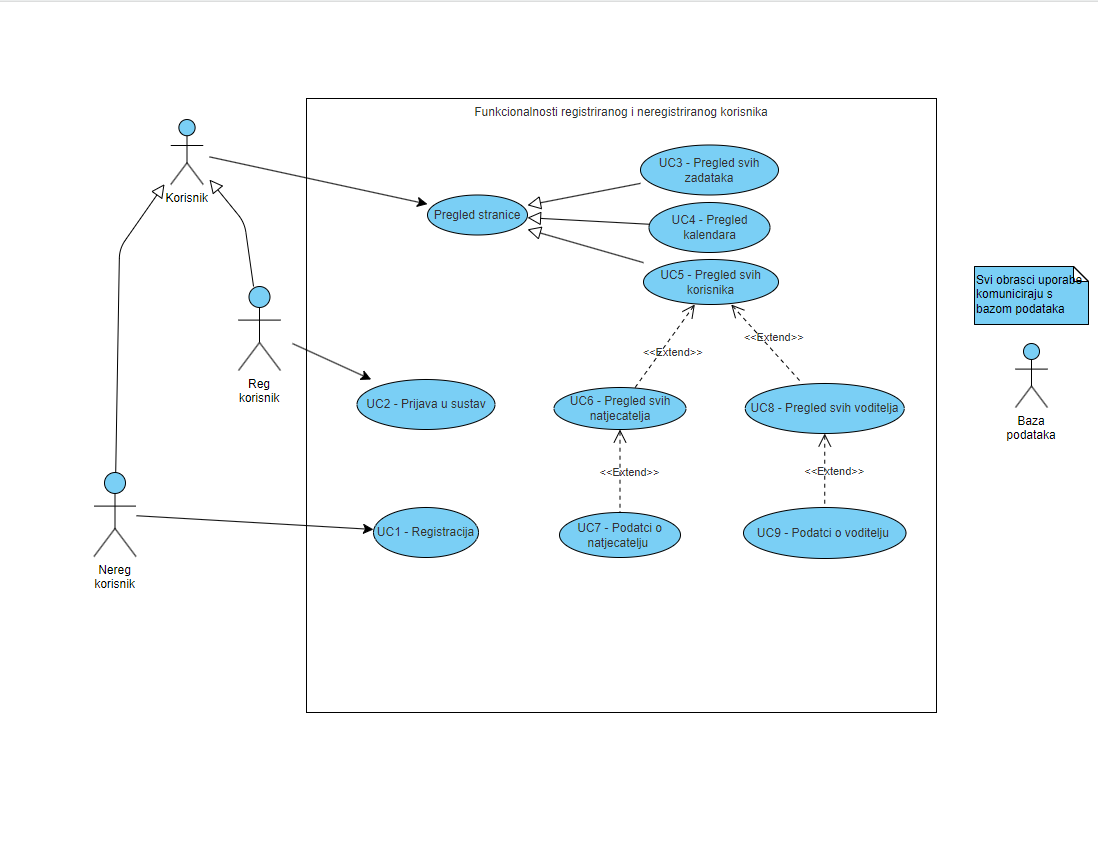
\includegraphics[scale=0.4]{slike/Uml - obrasci uporabe 1}
						%veličina slike u odnosu na originalnu datoteku i pozicija slike
						\centering
						\caption{Dijagram obrasca uporabe, funkcionalnost reg. i nereg. korisnika}
						\label{fig:dijagram1}
					\end{figure}
					
					\begin{figure}[H]
						\includegraphics[scale=0.4]{slike/Uml - obrasci uporabe 2}
						%veličina slike u odnosu na originalnu datoteku i pozicija slike
						\centering
						\caption{Dijagram obrasca uporabe, funkcionalnost voditelja, natjecatelja i administratora}
						\label{fig:dijagram2}
					\end{figure}
					
				\eject		
				
			\subsection{Sekvencijski dijagrami}
				
				\textbf{\textit{dio 1. revizije}}\
							
				
				\subsubsection{1) Registracija korisnika}
				
				\textbf{Opis dijagrama:}
				Korisnik započinje registraciju odabirom opcije "Registracija" na korisničkom sučelju. Nakon što korisnik odabere tu opciju, poslužitelj aplikacije šalje zahtjev korisniku da unese sljedeće podatke:
				
				\begin{itemize}
					\item (a) korisničko ime
					\item (b) fotografiju
					\item (c) lozinku
					\item (d) ime i prezime
					\item (e) email adresu
					\item (f) odabir: voditelj natjecanja / natjecatelj
				\end{itemize}
				
				Nakon što korisnik unese navedene podatke, potvrđuje svoju registraciju putem korisničkog sučelja. Nakon toga, poslužitelj provjerava unesene podatke. Prvo se provjerava dostupnost e-mail adrese u bazi podataka. U slučaju da je e-mail adresa već zauzeta, poslužitelj obavještava korisnika da registracija nije uspjela. U slučaju da je e-mail adresa dostupna, korisniku se šalje zahtjev za potvrdom registracije putem e-maila. Iz tog slučaja proizlaze dva nova scenarija:
				
				\begin{enumerate}
					\item Korisnik potvrđuje registraciju - novi podaci se pohranjuju u bazu podataka, a poslužitelj obavještava korisnika da je registracija uspješna.
					\item Korisnik ne potvrđuje registraciju - poslužitelj obavještava korisnika da registracija nije uspjela.
				\end{enumerate}
				
				U slučaju da je e-mail adresa dostupna, ali korisnik se registrira kao "voditelj natjecanja," tada se e-mail zahtjev za potvrdom registracije šalje administratoru, a ne korisniku. Iz tog slučaja proizlaze dva scenarija:
				
				\begin{enumerate}
					\item Administrator potvrđuje registraciju - novi podaci se pohranjuju u bazu podataka, a poslužitelj obavještava korisnika da je registracija uspješna.
					\item Administrator ne potvrđuje registraciju - poslužitelj obavještava korisnika da registracija nije uspjela.
				\end{enumerate}
				
				\textbf{Slika dijagrama:}
				\begin{figure}[H]
					\centering

					\caption{Sekvencijski dijagram registracije korisnika.}
				\end{figure}
				
				\subsubsection{2) Pregled i uređivanje korisnika}
				
				\textbf{Opis dijagrama:}
				Administrator šalje zahtjev za pregled korisnika i njihovih podataka tako da klikne na link "Pregled svih korisnika". Poslužitelj šalje upit bazi podataka za podatke registriranih korisnika, a baza podataka vraća podatke o registriranim korisnicima. Otvara se stranica s popisom registriranih korisnika i njihovim podacima koje je moguće urediti. Kada administrator pošalje zahtjev za izmjenom podataka nekog korisnika, baza podataka provjerava je li narušen integritet jedinstvenosti, odnosno je li administrator promijenio korisničko ime u drugo korisničko ime koje već postoji u bazi podataka. Iz ovog scenarija proizlaze dva slučaja:
				
				\begin{enumerate}
					    \item Promjenom nije narušen integritet - novi podaci se pohranjuju u bazu podataka. Administratoru se javlja da je promjena uspješna, te se istovremeno šalje e-mail putem mail-poslužitelja korisniku s njegovim novim podacima.
					\item Promjenom je narušen integritet - administratoru se javlja da promjena nije uspjela (korisničko ime već postoji u bazi podataka), te se traži ponovni unos podataka.
					\end{enumerate}
					
					\textbf{Slika dijagrama:}
					\begin{figure}[H]
					\centering

					\caption{Sekvencijski dijagram pregleda i uređivanja korisnika.}
					\end{figure}
					
					\subsubsection{3) Virtualno natjecanje}
					
					\textbf{Opis dijagrama:}
					Kada natjecatelj klikne na link/gumb "Virtualno natjecanje", poslužitelj mu nudi mogućnost odabira između "Prethodno natjecanje" i "Nasumično generirani zadaci".
					
					Ako natjecatelj odabere "Prethodno natjecanje", poslužitelj ga preusmjerava na kalendar natjecanja, gdje natjecatelj može birati samo natjecanja na kojima je već sudjelovao. Kada natjecatelj odabere određeno natjecanje, poslužitelj komunicira s bazom podataka kako bi provjerio je li natjecatelj sudjelovao na tom natjecanju. Iz tog scenarija proizlaze dva slučaja:
					
					\begin{enumerate}
					\item Natjecatelj nije prethodno sudjelovao na odabranom natjecanju, pa mu poslužitelj onemogućava pristup, te natjecatelj može odabrati drugo natjecanje.
					\item Natjecatelj je prethodno sudjelovao na natjecanju, te mu je omogućen pristup. Na kraju Virtualnog natjecanja, natjecateljev virtualni rezultat uspoređuje se s rang listom stvarnog natjecanja (čije podatke poslužitelj dohvaća iz baze podataka), i rezultat se prikazuje natjecatelju.
					\end{enumerate}
					
					Ako natjecatelj odabere opciju "Nasumično generirani zadaci", poslužitelj iz baze podataka dohvaća zadatke i generira ih ravnomjerno prema težini. Nakon generiranja zadataka, zadaci se prikazuju natjecatelju.
					
					\textbf{Slika dijagrama:}
					\begin{figure}[H]
					\centering
					
					\caption{Sekvencijski virtualnog natjecanja.}
					\end{figure}
			
					
				
				
	
		\section{Ostali zahtjevi}
		
			\textbf{\textit{dio 1. revizije}}\\
		 
			 \textit{Nefunkcionalni zahtjevi i zahtjevi domene primjene dopunjuju funkcionalne zahtjeve. Oni opisuju \textbf{kako se sustav treba ponašati} i koja \textbf{ograničenja} treba poštivati (performanse, korisničko iskustvo, pouzdanost, standardi kvalitete, sigurnost...). Primjeri takvih zahtjeva u Vašem projektu mogu biti: podržani jezici korisničkog sučelja, vrijeme odziva, najveći mogući podržani broj korisnika, podržane web/mobilne platforme, razina zaštite (protokoli komunikacije, kriptiranje...)... Svaki takav zahtjev potrebno je navesti u jednoj ili dvije rečenice.}
			 
			 
			 
	